\section{Diagrama de Actividades}%
\label{sec:diagrama_actividades} % Etiqueta para referencia cruzada

La representación explícita del flujo de trabajo operativo es fundamental para el diseño, la implementación y la validación del sistema propuesto en este trabajo. Dicho sistema integra técnicas de optimización bioinspiradas con simulaciones gravitacionales de N-cuerpos, utilizando la biblioteca REBOUND y abordando inicialmente el caso de dos cuerpos. La comprensión detallada de la secuencia de actividades, las bifurcaciones lógicas y la interacción entre los componentes clave —\textit{Usuario}, \textit{Interfaz de Usuario}, \textit{Motor de Optimización} (Algoritmo Bioinspirado), \textit{Simulador} (REBOUND) y \textit{Módulo de Visualización}— resulta esencial para gestionar la complejidad inherente a esta integración metodológica.

El diagrama de actividades presentado en la Sección~\ref{subsec:activity_diagram_img} sirve como una representación formal de este proceso dinámico. Modela cómo el algoritmo bioinspirado gestiona la generación de conjuntos de parámetros, inicia ejecuciones de simulación en REBOUND y evalúa los resultados para refinar iterativamente la búsqueda de soluciones que satisfagan criterios predefinidos (p.\ ej., estabilidad orbital).

Mediante la descomposición del proceso global en pasos discretos y la asignación de responsabilidades a través de carriles (swimlanes), el diagrama clarifica la lógica operativa y establece una base para una implementación estructurada y verificable. Asegura que la integración del ciclo de optimización con el motor de simulación sea coherente con los objetivos del proyecto, facilitando el desarrollo de una solución robusta para la exploración de escenarios de N-cuerpos bajo criterios de optimización específicos.

\subsection{Diagrama de Actividades}%
\label{subsec:activity_diagram_img}

A continuación, se presenta el diagrama de actividades que modela el flujo operativo del sistema, abarcando la optimización de parámetros mediante algoritmos bioinspirados y la ejecución de simulaciones N-cuerpos con REBOUND.\

\begin{figure}[H] % Opciones de posicionamiento: here, top, bottom, page
    \centering
    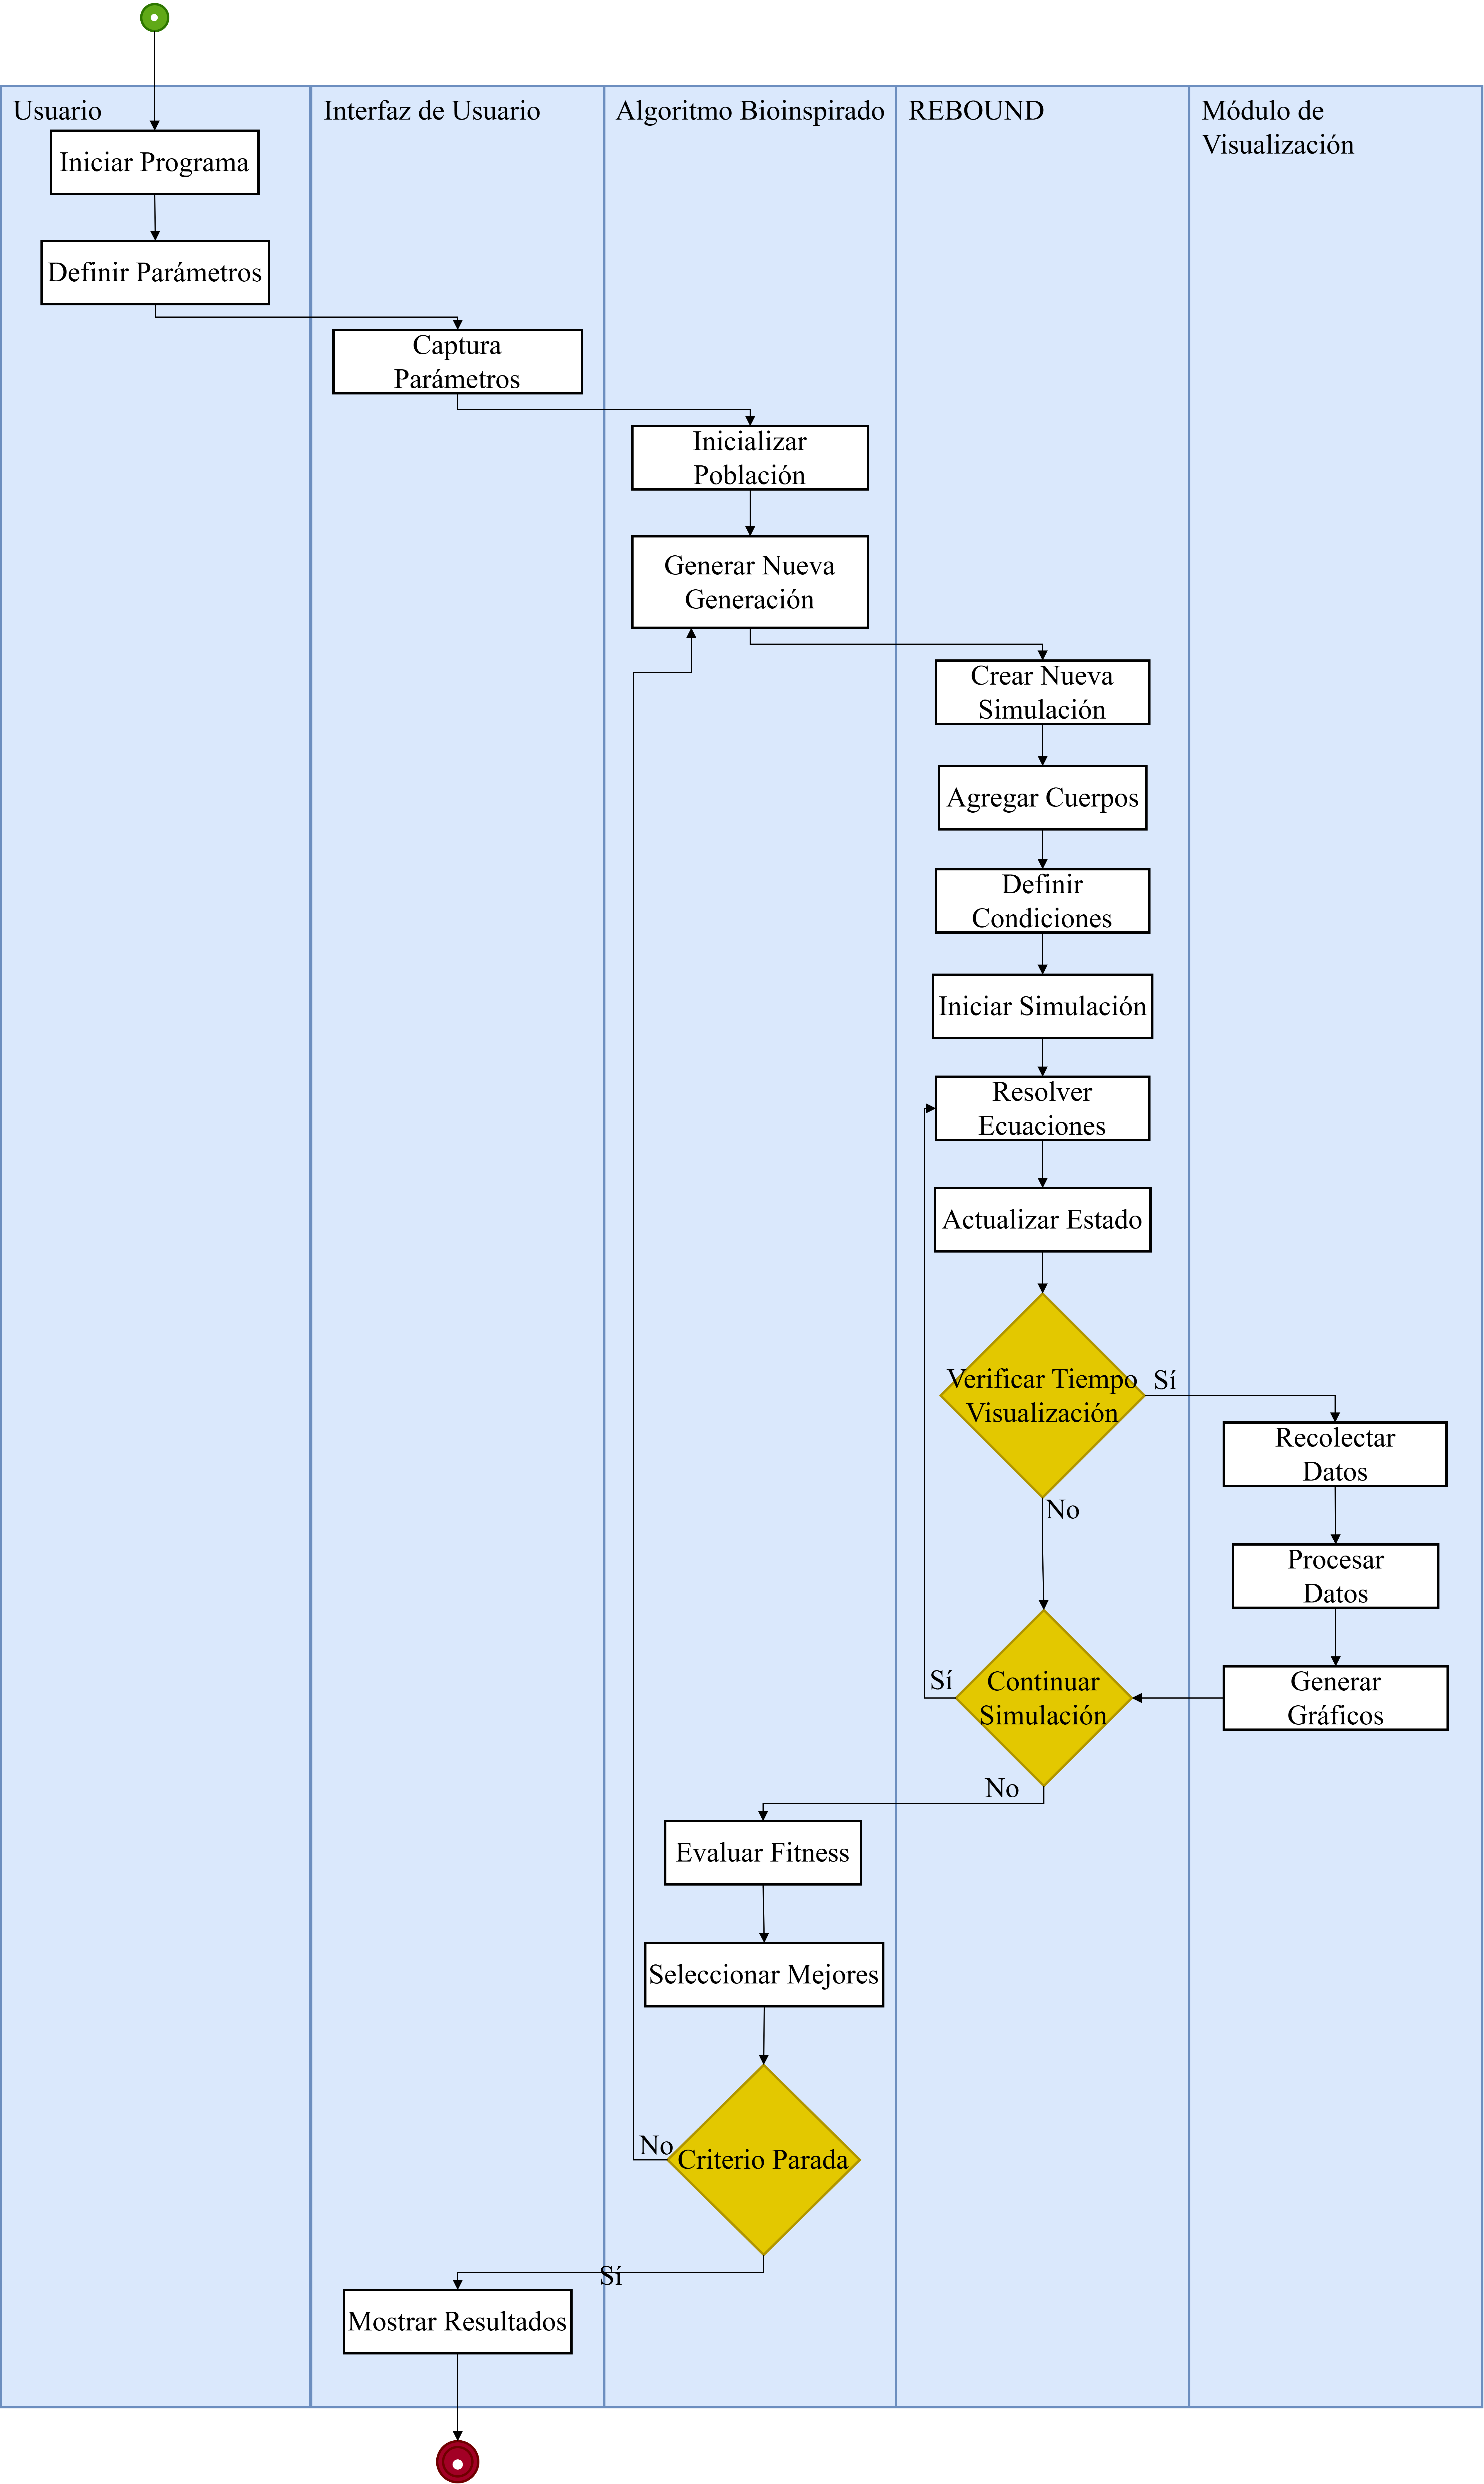
\includegraphics[width=\textwidth]{img/Analisis/DiagramaActividades2.png}
    \caption{Diagrama de Actividades UML del proceso de simulación y optimización.}%
    \label{fig:activity_diagram} % Etiqueta para referenciar la figura
\end{figure}

\subsection{Descripción del Diagrama de Actividades}

\subsubsection{Estructura del Diagrama: Carriles (Swimlanes)}

El diagrama se organiza en cinco carriles (swimlanes), cada uno representando un actor o componente lógico del sistema, delineando sus responsabilidades específicas:

\begin{enumerate}
    \item \textbf{Usuario:} Representa al actor humano que interactúa con el sistema. Es responsable de iniciar la ejecución y proporcionar la configuración inicial requerida.
    \item \textbf{Interfaz de Usuario (UI):} Componente software que media la interacción entre el \textit{Usuario} y el núcleo del sistema. Gestiona la captura de parámetros de entrada y la presentación de resultados.
    \item \textbf{Algoritmo Bioinspirado:} Componente central responsable de la optimización. Administra la población de soluciones candidatas (conjuntos de parámetros), aplica operadores evolutivos (generación, evaluación, selección) y determina la terminación del proceso según criterios definidos.
    \item \textbf{REBOUND:} Representa la biblioteca de simulación gravitacional. Ejecuta simulaciones de N-cuerpos (inicialmente, 2 cuerpos) basadas en los parámetros proporcionados por el \textit{Algoritmo Bioinspirado} para cada individuo evaluado. Cabe destacar que se instancia una nueva simulación para cada conjunto de parámetros a evaluar.
    \item \textbf{Módulo de Visualización:} Componente encargado de generar representaciones gráficas del estado del sistema en instantes de tiempo específicos, definidos por el \textit{Usuario}, para el monitoreo de la evolución dinámica.
\end{enumerate}

\subsubsection{Flujo Detallado de Actividades}

El proceso modelado en el diagrama sigue la secuencia lógica que se describe a continuación:

\begin{enumerate}
    \item \textbf{Inicialización y Configuración:}
        \begin{itemize}
            \item El \textit{Usuario} inicia la ejecución de la aplicación (\textbf{Iniciar Programa}).
            \item El \textit{Usuario} especifica los parámetros de configuración inicial, incluyendo rangos de búsqueda para la optimización, la función objetivo, criterios de parada, y los instantes discretos de tiempo para la visualización (\textbf{Definir Parámetros}).
            \item La \textit{Interfaz de Usuario} captura y valida esta información (\textbf{Captura Parámetros}).
        \end{itemize}

    \item \textbf{Ciclo Iterativo de Optimización y Simulación:}
        \begin{itemize}
            \item La \textit{UI} transmite los parámetros de configuración al \textit{Algoritmo Bioinspirado}, el cual inicializa su población de soluciones candidatas (\textbf{Inicializar Población}).
            \item \textbf{Inicio del Bucle de Optimización:} El algoritmo genera una nueva generación de conjuntos de parámetros candidatos aplicando sus operadores definidos (\textbf{Generar Nueva Generación}).
            \item \textbf{Ejecución de Simulaciones por Individuo:} Para cada conjunto de parámetros (individuo) en la generación actual:
                \begin{itemize}
                    \item Se instruye a \textit{REBOUND} para crear una nueva instancia de simulación (\textbf{Crear Nueva Simulación}).
                    \item Se añaden los cuerpos celestes al entorno de simulación con las propiedades especificadas por el conjunto de parámetros actual (\textbf{Agregar Cuerpos}).
                    \item Se configuran las condiciones restantes de la simulación, como el integrador numérico y el paso de tiempo (\textbf{Definir Condiciones}).
                    \item \textit{REBOUND} inicia la simulación (\textbf{Iniciar Simulación}).
                    \item \textbf{Bucle Interno de Simulación (REBOUND):}
                        \begin{itemize}
                            \item \textit{REBOUND} resuelve las ecuaciones de movimiento para avanzar un paso de tiempo (\textbf{Resolver Ecuaciones}).
                            \item Actualiza el estado del sistema (posiciones, velocidades) (\textbf{Actualizar Estado}).
                            \item Verifica si el tiempo de simulación actual ($t_{\text{sim}}$) corresponde a uno de los instantes de visualización solicitados ($t_{\text{vis}}$) (\textbf{Verificar Tiempo Visualización}).
                            \item Si $t_{\text{sim}} = t_{\text{vis}}$ (Condición Verdadera): Se activa el \textit{Módulo de Visualización}, que recolecta los datos relevantes del estado actual (\textbf{Recolectar Datos}), los procesa (\textbf{Procesar Datos}) y genera la salida gráfica correspondiente (\textbf{Generar Gráficos}). La simulación continúa.
                            \item Si $t_{\text{sim}} \neq t_{\text{vis}}$ (Condición Falsa): La simulación continúa directamente al siguiente paso.
                            \item \textit{REBOUND} verifica si se ha alcanzado la condición de término de la simulación (p.\ ej., tiempo final $T_{\text{max}}$) (\textbf{Continuar Simulación}). Si no se ha alcanzado (Condición Falsa), retorna a \textbf{Resolver Ecuaciones}. Si se ha alcanzado (Condición Verdadera: \textbf{Simulación Terminada}), la ejecución para este individuo finaliza.
                        \end{itemize}
                \end{itemize}
            \item \textbf{Evaluación:} Tras la finalización de la simulación para un individuo, el \textit{Algoritmo Bioinspirado} utiliza los resultados (p.\ ej., una métrica derivada del estado final o la trayectoria) para calcular su valor de aptitud (fitness) (\textbf{Evaluar Fitness}). Este paso se repite para todos los individuos de la generación.
            \item \textbf{Selección y Criterio de Parada:} El \textit{Algoritmo Bioinspirado} aplica sus mecanismos de selección basados en la aptitud calculada (\textbf{Seleccionar Mejores}) y verifica si se cumple el criterio global de parada (p.\ ej., número máximo de generaciones, convergencia de la aptitud) (\textbf{Criterio Parada}).
                \begin{itemize}
                    \item Si el criterio no se cumple (Condición Falsa): Se procede a generar la siguiente generación (\textbf{Generar Nueva Generación}), continuando el ciclo de optimización.
                    \item Si el criterio se cumple (Condición Verdadera): El ciclo de optimización concluye.
                \end{itemize}
        \end{itemize}

    \item \textbf{Finalización:}
        \begin{itemize}
            \item El \textit{Algoritmo Bioinspirado} transfiere la mejor solución encontrada (conjunto de parámetros óptimos y su aptitud asociada) a la \textit{Interfaz de Usuario}.
            \item La \textit{Interfaz de Usuario} presenta los resultados finales al \textit{Usuario} (\textbf{Mostrar Resultados}).
            \item El proceso finaliza (nodo final de actividad). % O referenciar el símbolo específico si se usa en el diagrama
        \end{itemize}
\end{enumerate}

\subsection{Aspectos Clave del Diseño Reflejados en el Diagrama}

El diagrama de actividades pone de manifiesto varios aspectos fundamentales del diseño del sistema:

\begin{itemize}
    \item \textbf{Modularidad y Separación de Responsabilidades:} La estructura en carriles delimita claramente las funciones del componente de optimización (\textit{Algoritmo Bioinspirado}) y del componente de simulación física (\textit{REBOUND}), promoviendo un diseño modular.
    \item \textbf{Naturaleza Iterativa del Proceso:} El bucle principal que engloba \textbf{Generar Nueva Generación}, la ejecución de simulaciones en \textit{REBOUND}, \textbf{Evaluar Fitness} y \textbf{Criterio Parada} representa visualmente el núcleo iterativo característico de los algoritmos evolutivos y otros métodos de optimización bioinspirados.
    \item \textbf{Simulación como Evaluación de Aptitud:} Desde la perspectiva del optimizador, el módulo \textit{REBOUND} actúa como una función objetivo (o parte de ella), evaluando la calidad (aptitud) de un conjunto de parámetros candidato mediante la ejecución de una simulación física.
    \item \textbf{Instanciación Independiente de Simulaciones:} El flujo muestra que cada evaluación de un individuo dentro del ciclo de optimización requiere la creación y ejecución de una nueva instancia de simulación en \textit{REBOUND}, configurada con los parámetros específicos de dicho individuo.
    \item \textbf{Control Discreto de la Visualización:} La generación de visualizaciones está integrada en el bucle de simulación de \textit{REBOUND} pero se activa únicamente en puntos temporales discretos especificados por el \textit{Usuario}, evitando una sobrecarga continua.
\end{itemize}
